\begin{frame}[fragile,t]{\secname}%{\subsecname}

\begin{itemize}
 \item RVE: Initial attempt with tet mesh and critical stretch model
\end{itemize}

% \begin{center}
\begin{minipage}[t][0.7\textheight][t]{0.49\textwidth}
  \centering
  \IfFileExists{Videos/RVE_Fatigue_r113360_dam_R3_nolegend.mp4}{
  \only<1|handout:0>{
		\begin{tikzpicture}
		  % Axis style
		  \pgfplotsset{
			myperidigmdamageaxis style/.style={
			  hide axis,
			  scale only axis,
			  point meta min=0.0,                       % Minimum value colorbar
			  point meta max=0.5,                       % Maximum value colorbar
			  tick label style={font=\figurefontsize},  
			  %colormap/bluered,                         % Colormap preset
			}
		  }
		  % Video
		%   \begin{pgfonlayer}{layervideo}
		%     \node (video) {
		%       \includemedia[
		%         height=0.7\textheight,
		%         width=0.9\textwidth,
		%         keepaspectratio,
		%         activate=pageopen,
		%         addresource=Videos/RVE_Fatigue_r113360_udam_R3.mp4,
		%         flashvars={source=Videos/RVE_Fatigue_r113360_udam_R3.mp4}
		%         ]{}{VPlayer.swf}%{VPlayer9.swf}
		%     };
			\node (video1) {
			  \includemedia[
				height=0.65\textheight,
				width=0.7\linewidth,
				keepaspectratio,
				activate=pageopen,
				addresource=Videos/RVE_Fatigue_r113360_dam_R3_nolegend.mp4,
				flashvars={source=Videos/RVE_Fatigue_r113360_dam_R3_nolegend.mp4}
				]{}{VPlayer.swf}%{VPlayer9.swf}
			};
		  % Colorbar right
			\begin{axis}[%
			  myperidigmdamageaxis style,
	  %         %at={(video.east)},
	  %         %anchor=west,
			  at={(video1.west)},
			  anchor=east,
			  height=0.65\textheight,
			  xshift=3.0cm,                              % Adjust this for horizontal sep
			  colorbar left,                             % Activate colorbar
			  colorbar sampled,
			  colormap name=paraviewblueredcolormap,
			  colorbar style={
				paraviewdiscrete256colorbar style,
				%ylabel=Damage variable [-],             % Label
				ylabel=Damage [-],                       % Label
				y label style={
				  at={(2em,1.075)},
				  rotate=-90,
				},
				label style={font=\figurefontsize},
				scaled y ticks=false,
			  },
			]
			  \addplot [draw=none] coordinates {(0,0)}; % Dummy plot
			\end{axis}
		\end{tikzpicture}
	  }
	  \only<2|handout:1>{
		\hspace{2em}
		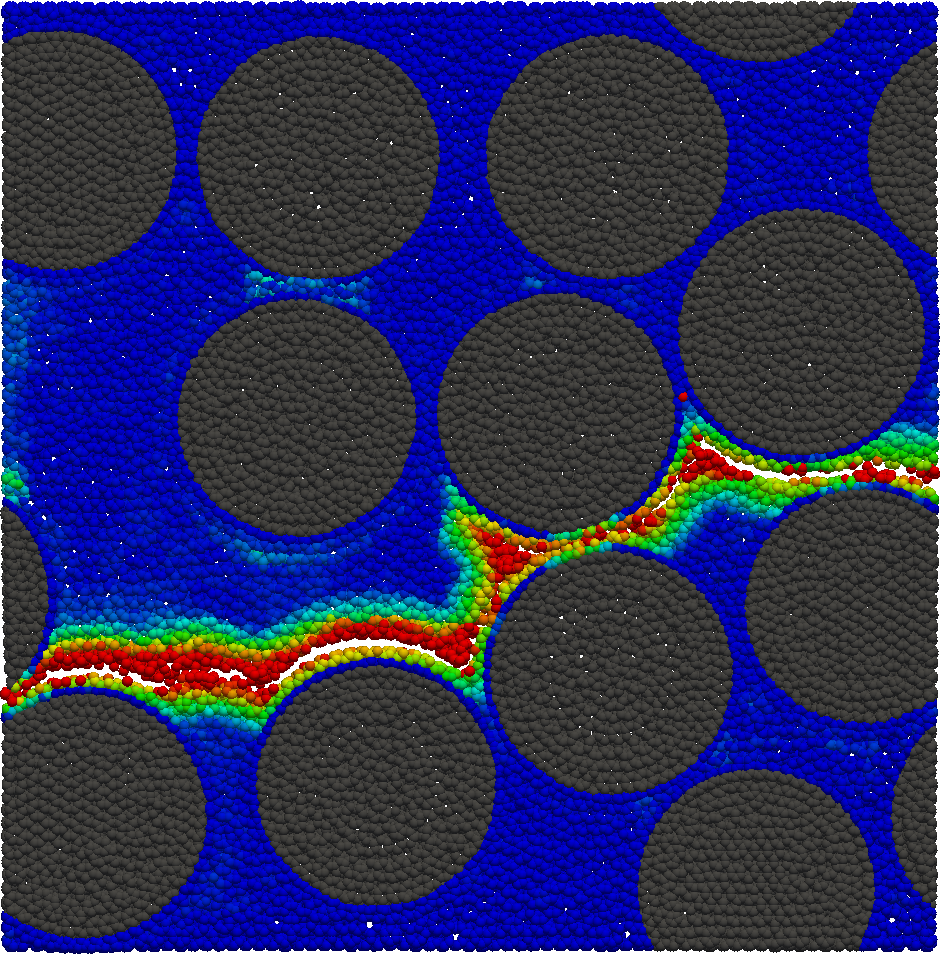
\includegraphics[width=\linewidth,height=0.65\textheight,keepaspectratio]{PD_RVE_Fatigue_r113360_dam_R3_nolegend_2400_1000px_ct.png}
	  }
	}{
	  \only<1|handout:1>{
		\hspace{2em}
		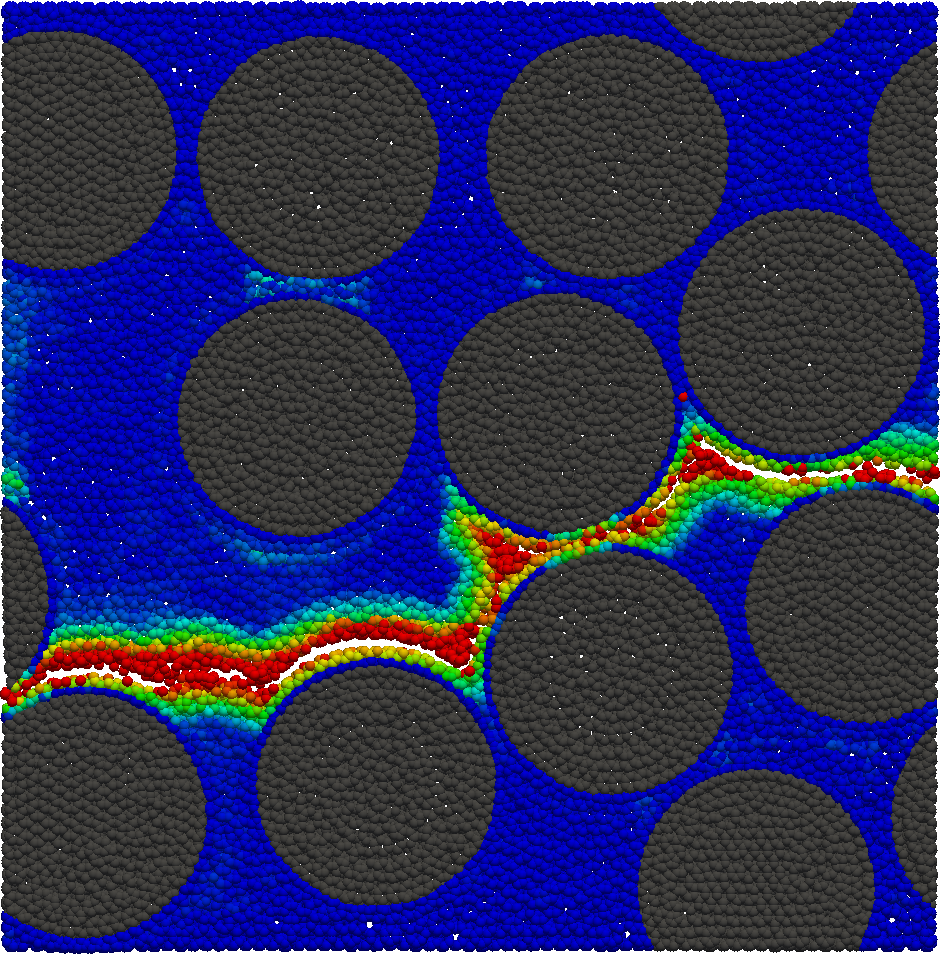
\includegraphics[width=\linewidth,height=0.65\textheight,keepaspectratio]{PD_RVE_Fatigue_r113360_dam_R3_nolegend_2400_1000px_ct.png}
	  }
	
	}
\end{minipage}
\begin{minipage}[t][0.7\textheight][t]{0.49\textwidth}
  \IfFileExists{Videos/RVE_Fatigue_r113360_dam_R3_nolegend.mp4}{
	  %\includegraphics[width=\linewidth]{example-image-a}
	  \only<1|handout:0>{
		\begin{tikzpicture}
		  % Axis style
		  \pgfplotsset{
			mydisplacementaxis style/.style={
			  hide axis,
			  scale only axis,
			  point meta min=0.0,                       % Minimum value colorbar
			  point meta max=0.04,                       % Maximum value colorbar
			  tick label style={font=\figurefontsize},  
			  %colormap/bluered,                         % Colormap preset
			  %colorbar sampled,                         % Steps in colorbar
			}
		  }
		  % Layers
		%   \pgfdeclarelayer{layervideo}
		%   \pgfdeclarelayer{layercolorbar}
		%   \pgfsetlayers{layervideo,layercolorbar}
		  % Video
		%     \node (video) {
		%       \includemedia[
		%         height=0.7\textheight,
		%         width=0.9\textwidth,
		%         keepaspectratio,
		%         activate=pageopen,
		%         addresource=Videos/RVE_Fatigue_r113360_udam_R3.mp4,
		%         flashvars={source=Videos/RVE_Fatigue_r113360_udam_R3.mp4}
		%         ]{}{VPlayer.swf}%{VPlayer9.swf}
		%     };
			\node (video2) {
			  \includemedia[
				height=0.65\textheight,
				width=0.7\linewidth,
				keepaspectratio,
				activate=pageopen,
				addresource=Videos/RVE_Fatigue_r113360_u_R3_nolegend.mp4,
				flashvars={source=Videos/RVE_Fatigue_r113360_u_R3_nolegend.mp4}
				]{}{VPlayer.swf}%{VPlayer9.swf}
			};
		  % Colorbar right
			\begin{axis}[%
			  mydisplacementaxis style,
			  %at={(video.east)},
			  %anchor=west,
			  at={(video2.east)},
			  anchor=west,
			  height=0.65\textheight,
			  xshift=-3.0cm,
			  colorbar right,                           % Activate colorbar
			  colorbar sampled,
			  colormap name=paraviewblueredcolormap,
			  colorbar style={
				paraviewdiscrete256colorbar style,
				%ylabel=Damage variable [-],             % Label
				ylabel={$u_y$ $\si{\milli\meter}$},      % Label
				y label style={
				  at={(-1em,1.075)},
				  rotate=-90,
				},
				label style={font=\figurefontsize},
				yticklabel style={
				  /pgf/number format/fixed,
				  /pgf/number format/precision=2,
				},
				scaled y ticks=false,
			  },
			]
			  \addplot [draw=none] coordinates {(0,0)}; % Dummy plot
			\end{axis}
		\end{tikzpicture}
	  }
	  \only<2|handout:1>{
		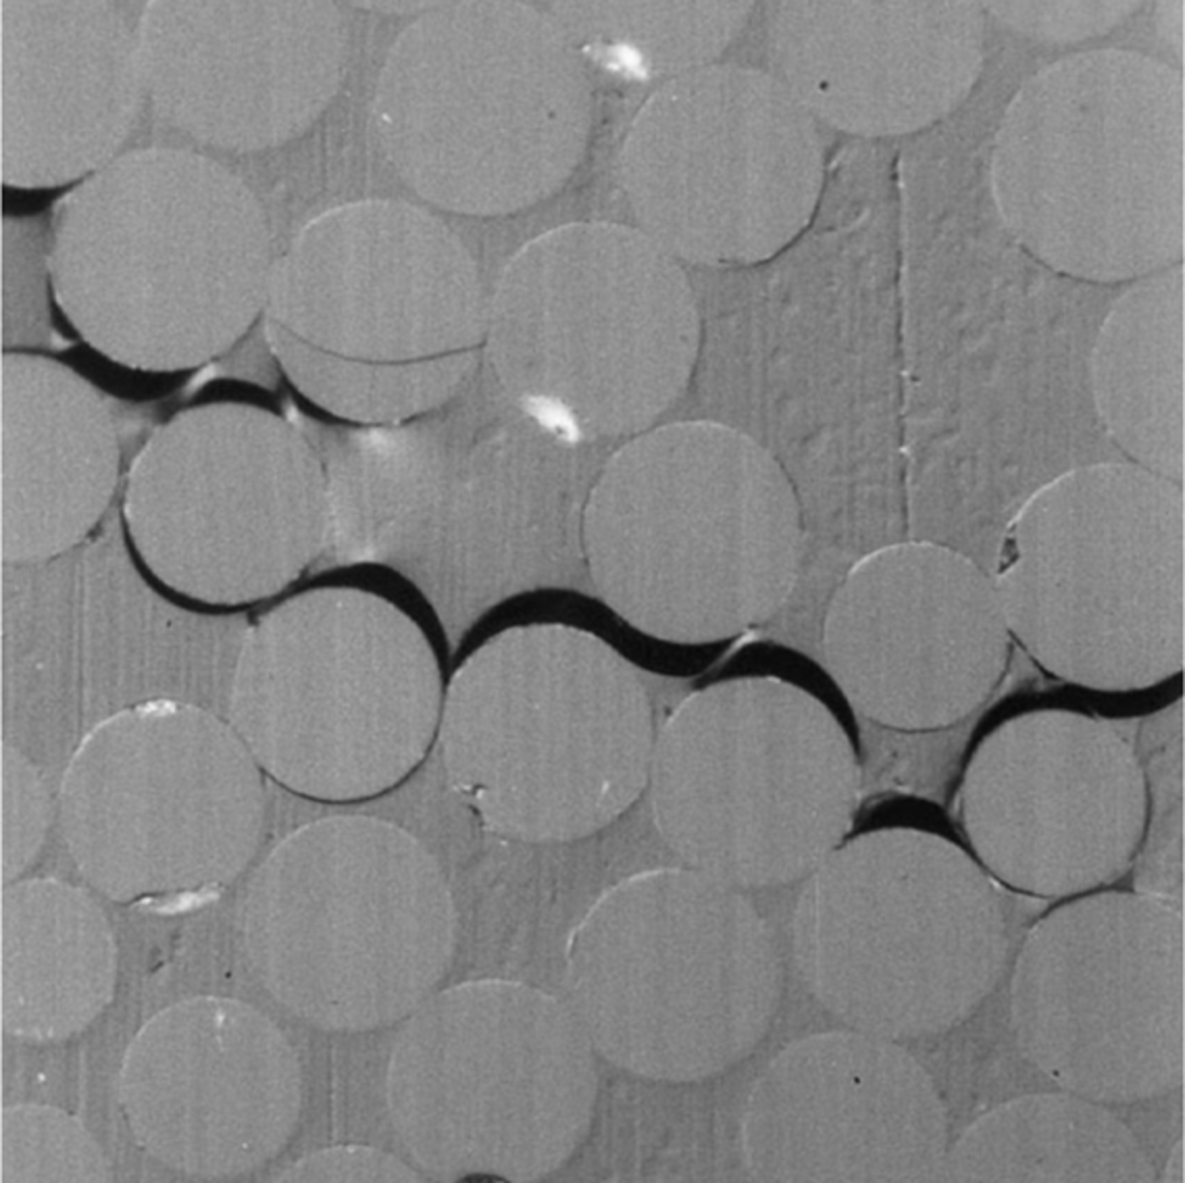
\includegraphics[width=\linewidth,height=0.65\textheight,keepaspectratio]{Exp_Matrix_Failure}
	  }
	}{
	  \only<1|handout:1>{
		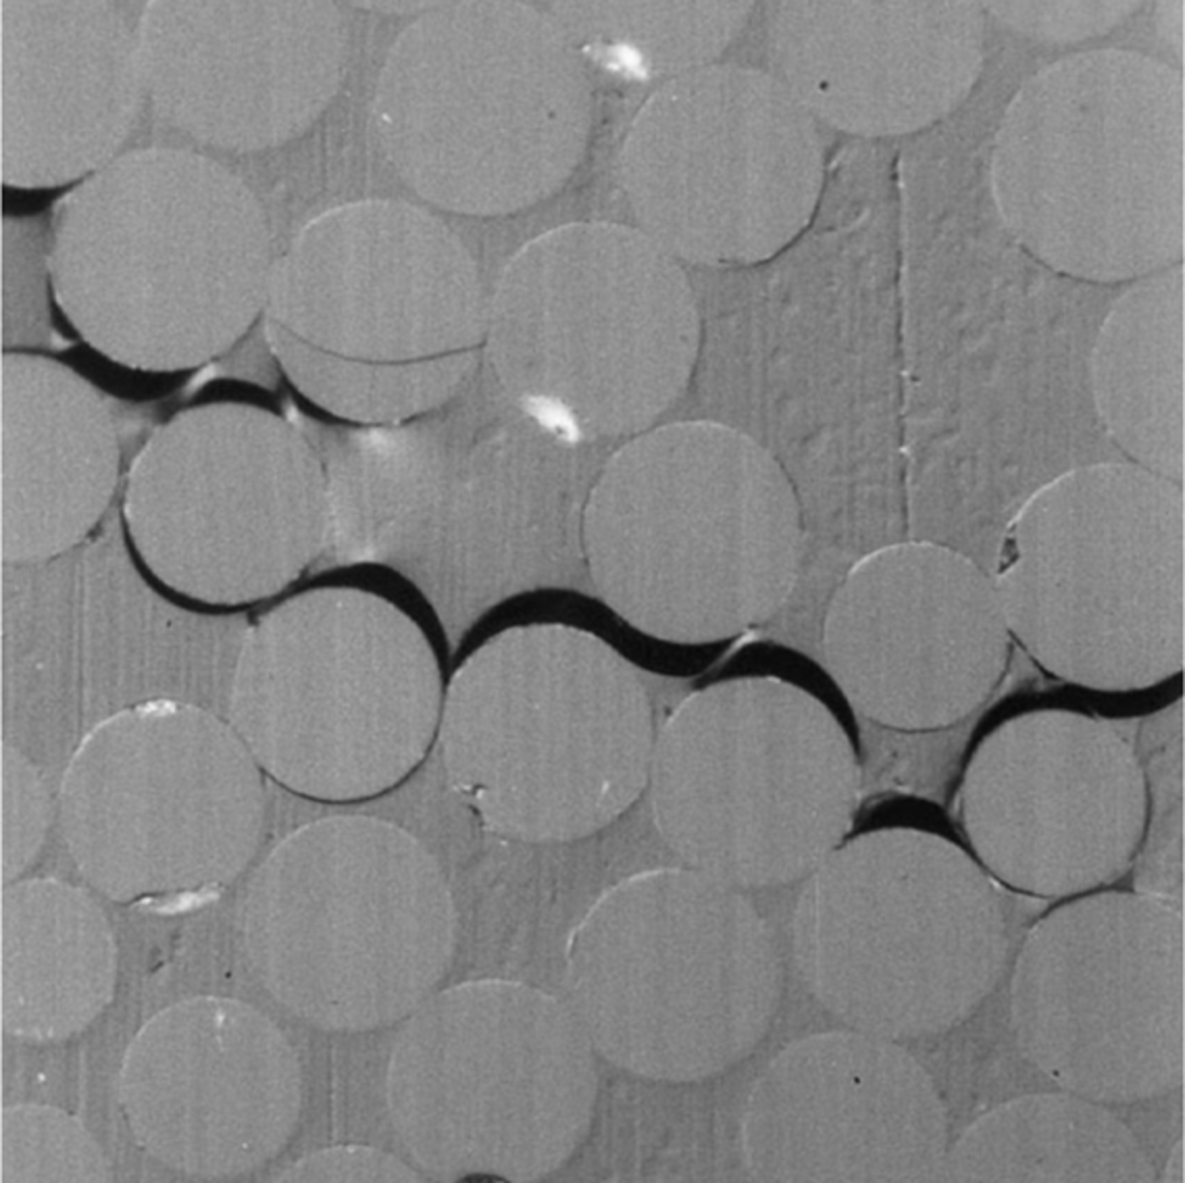
\includegraphics[width=\linewidth,height=0.65\textheight,keepaspectratio]{Exp_Matrix_Failure}
	  }
	}
\end{minipage}

% \end{center}

\end{frame}
